\chapter{Commercial Real Estate Brokers Advice To Young People}

This short interview is not a blackboard lecture, but it does have a clean argumentative spine. We begin with self-command, pass through the handling of money, and only then arrive at commercial real estate as a relationship market. Since no validated visual mathematics survives for this chapter, every formal expression below should be read as a cautious transcript-backed reconstruction of the speaker's method rather than as a literal board transcription.

\section{Personal Discipline Before Strategy}

The opening question is retrospective: what would one tell the twenty-year-old self? The answer is deliberately harsh. Before we are given a market, a sector, or a tactic, we are given a prior condition: get organized, stop wasting time, stop being late to seriousness. That is the correct opening for the chapter, because the later commercial advice is not presented as a trick for making money; it is presented as something that only becomes available once disorder has been reduced.

In this sense the lecture begins with a primitive variable that is never written on the board but is everywhere assumed: sustained effort. If effort is scattered, everything downstream is weakened. If effort is concentrated, later opportunities have something to attach themselves to.

We may summarize the opening logic schematically as
\begin{equation}
\text{discipline} \to \text{sustained effort}.
\end{equation}
This is not a quoted formula. It is the simplest faithful compression of the first movement of the interview.

\section{Early Money and the Consumption Trap}

The next move is to give self-disorder a more concrete shape. The speaker does not leave the matter at vague exhortation. He names the distractions: chasing girls, drinking beer, and then, once money arrives, rushing to buy the flashy car. The lecture is careful here. It is not anti-money. It is anti-dissipation.

That distinction is worth preserving. A rise in income is not, by itself, a command to expand status consumption. The warning is sharp precisely because it comes in the register of ordinary behavior rather than abstract finance.

A minimal way to record the point is
\begin{equation}
Y \uparrow \not\Rightarrow C_s \uparrow,
\end{equation}
where \(Y\) is income and \(C_s\) denotes conspicuous or status-oriented consumption. The chapter should not pretend that the speaker offered a utility theory; he did not. But he did plainly deny the inference from earning more to spending more on vanity.

We can make the same point in prose: money earned is not yet wealth secured. The moral and the commercial lines coincide here. What leaks attention also leaks capital.

\section{Credibility and the Choice of Industry}

The interviewer then asks a question that functions as a hinge: what was the most money made in a single year? The answer is intentionally rough but quantitative enough to matter:
\begin{equation}
10^6 \le Y < 10^7.
\end{equation}
The phrase is ``in the seven digits,'' so we should preserve only the interval and not invent an exact number.

This brief numerical claim does real structural work. It turns the earlier warning against waste into tested advice rather than pious advice. Only after that credibility marker does the interview ask the next necessary question: what industry produced that result? The answer is commercial real estate.

Now the lecture narrows. We are no longer in the broad territory of youth and regret. We are entering a market with a definite structure. The next question, therefore, is no longer moral but operational: how does one break in?

\section{Commercial Real Estate as a Relationship Market}

The speaker's first answer is not about spreadsheets, licensing exams, or macro forecasts. It is much simpler:
\begin{equation}
\text{commercial real estate entry} \to \text{relationship-based process}.
\end{equation}
This is the central proposition of the chapter.

To keep the later formalism disciplined, let us introduce a minimal vocabulary.

\begin{definition}
Fix a local market \(\mathcal{M}\). Let \(B(\mathcal{M})\) denote the set of buildings relevant to the beginner's chosen territory. Let \(L_t \subseteq B(\mathcal{M})\) denote the subset whose lobbies or premises have been physically covered by time \(t\). Let \(K_t\) denote the stock of practical local knowledge generated by that coverage, and let \(R_t\) denote the stock of relationships built from repeated presence and informed contact.
\end{definition}

The speaker's phrase ``know every building'' is best read against this local market \(\mathcal{M}\), not as a literal command to master an entire city at once. In notation,
\begin{equation}
L_t \subseteq B(\mathcal{M}), \qquad K_t = K(L_t),
\end{equation}
with the understanding that more coverage tends to produce more usable knowledge.

\begin{figure}
\centering
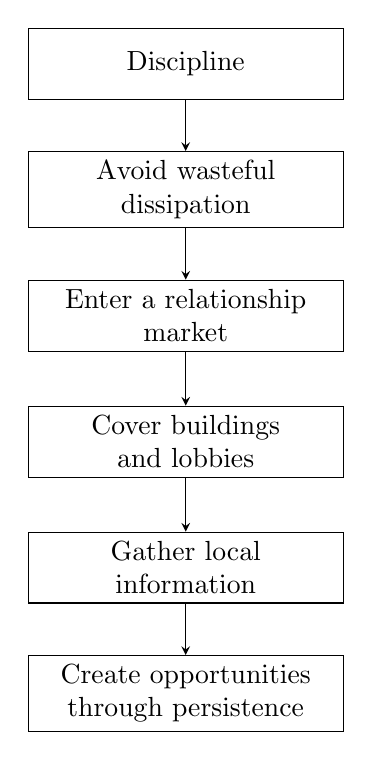
\begin{tikzpicture}[>=stealth]
\node[draw, rectangle, align=center, minimum width=4.0cm, minimum height=0.9cm] (a) at (0,0) {Discipline};
\node[draw, rectangle, align=center, minimum width=4.0cm, minimum height=0.9cm] (b) at (0,-1.6) {Avoid wasteful\\dissipation};
\node[draw, rectangle, align=center, minimum width=4.0cm, minimum height=0.9cm] (c) at (0,-3.2) {Enter a relationship\\market};
\node[draw, rectangle, align=center, minimum width=4.0cm, minimum height=0.9cm] (d) at (0,-4.8) {Cover buildings\\and lobbies};
\node[draw, rectangle, align=center, minimum width=4.0cm, minimum height=0.9cm] (e) at (0,-6.4) {Gather local\\information};
\node[draw, rectangle, align=center, minimum width=4.0cm, minimum height=0.9cm] (f) at (0,-8.0) {Create opportunities\\through persistence};

\draw[->] (a) -- (b);
\draw[->] (b) -- (c);
\draw[->] (c) -- (d);
\draw[->] (d) -- (e);
\draw[->] (e) -- (f);
\end{tikzpicture}
\end{figure}

This diagram is a schematic reconstruction from the transcript. It is included not as recovered lecture artwork but as a compact map of the lecture's own progression from conduct to commerce.

\subsection{Question \& Answer}

The interview naturally raises a question at this point. If the market is relationship-based, what must a beginner actually do? The danger in writing this chapter is to leave the answer at the level of slogan. The transcript does not do that. It immediately sharpens the idea.

The answer is not ``network'' in the soft modern sense. The answer is territorial and physical: know every building, be in the lobby of every building, and figure out what is happening there. In other words, relationships are not treated as detached social assets; they are byproducts of repeated, informed contact with a living market.

So the question is answered by converting a noun into a process:
\begin{equation}
\text{relationship} \;\; \text{is produced by} \;\; \text{coverage} + \text{presence} + \text{local knowledge}.
\end{equation}

\section{Territory Coverage as Commercial Method}

Once the question has been posed and answered, the lecture becomes operational. We are told to stand in lobbies, to observe, and to figure out what is going on inside buildings. The natural reconstruction is therefore an update rule. Let \(A_t\) denote the intensity of active fieldwork at step \(t\): visits, presence, follow-up, and repeated circulation through the market.

A minimal transcript-backed update model is
\begin{align}
K_{t+1} &= K_t + \alpha A_t, \\
R_{t+1} &= R_t + \beta A_t + \gamma K_t,
\end{align}
with \(\alpha,\beta,\gamma > 0\). The first line says that activity increases local knowledge. The second says that relationships are built by showing up, but also by showing up intelligently.

This is the right place for a worked derivation, because the interview itself unfolds the method step by step.

\paragraph{Worked derivation.}
\begin{enumerate}
\item We begin with a relationship market: entry depends on who knows us and what we know.
\item The speaker then specifies a physical program: visit buildings and stand in lobbies.
\item Each such act enlarges or refreshes the covered set \(L_t\), and hence raises \(K_t\).
\item Higher \(K_t\) makes contact more informed; informed contact builds \(R_t\).
\item Therefore activity does not merely consume time. It compounds into market knowledge and relationship stock.
\end{enumerate}

This is why the advice is concrete rather than inspirational. One does not wait for opportunity and then become active. One becomes active in order to generate the informational conditions under which opportunity can appear.

\begin{remark}
The update rules above are not quoted equations from the speaker. They are a restrained formalization of the spoken mechanism. The chapter should keep that distinction clear.
\end{remark}

\section{Opportunity, Refusal, and Persistence}

The final lines of the interview compress the entire method into two short claims: being busy creates opportunity, and a refusal should not be treated as final. Now we can see why those lines belong at the end. They are not free-floating encouragement. They are the summary of the mechanism already described.

Let \(O_t\) denote the flow of opportunities available at time \(t\). Then the lecture suggests the monotonic relation
\begin{equation}
O_t = f(K_t,R_t), \qquad \frac{\partial f}{\partial K} > 0, \qquad \frac{\partial f}{\partial R} > 0.
\end{equation}
Again, the point is not to fit a model. The point is to state as cleanly as possible what the lecture insists on verbally: more local knowledge and stronger relationships increase the possibility of useful openings.

The last line concerns refusal. Let \(N_t\) encode the event that a prospect, contact, or situation returns ``no.'' The lecture's operational rule is
\begin{equation}
N_t = 1 \Longrightarrow A_{t+1} \ge A_t.
\end{equation}
That is, rejection does not send activity to zero. At most it redirects the next step. We should hear the line ``don't take no for an answer'' in this local sense: do not collapse the search because one edge of the graph failed to open.

Putting the pieces together, the final causal chain is
\begin{equation}
A_t \to K_t \to R_t \to O_t,
\end{equation}
with persistence ensuring that the chain is not broken prematurely by ordinary friction.

\section{Summary}

The interview begins with character and ends with commercial method, and that order should be preserved. First we are told to stop wasting ourselves. Then we are told not to convert income into showy leakage. Only after that do we arrive at the credible claim of success, the naming of commercial real estate, and the governing principle that the business is relationship-based.

From there the chapter becomes almost geometric. We choose a market \(\mathcal{M}\), widen our coverage of its buildings, accumulate knowledge, turn that knowledge into relationships, and let opportunity emerge from sustained activity. The final maxims are therefore exact in their place: being busy creates opportunity, and refusal is not a command to stop.